\documentclass[simplex.tex]{subfiles}
% NO NEED TO INPUT PREAMBLES HERE
% packages are inherited; you can compile this on its own

\begin{document}
\subsection{ndmg}

Through use of the recently-developed cloud deployment options in ndmg, a collection of 3,000 human brain scans was
processed in a single day for under \$1,000 using our pipeline. The results are all publicly available online at our
website, \url{http://m2g.io}, and we have continued work on building a paper documenting our pipeline around this tool
and these exciting results. One such result, as shown in Figure~\ref{fig:ndmg_meanconnectome}, illustrates the mean
connectomes from a variety of datasets, and computes a multi-center mean and standard deviation connectome, as well.
This figure both illustrates the consistency of our pipeline across a wide range of data, and sheds light on properties
about the structure of the brain. Exploring these figures further, we can identify edges which are most highly variable
in the brain, and focus studies trying to understand the properties of the related regions lend themselves to such high
variability as opposed to other edges with lower variability.

\begin{figure}[h!]
\begin{cframed}[lgray]
\centering
\begin{subfigure}[h]{1\textwidth}
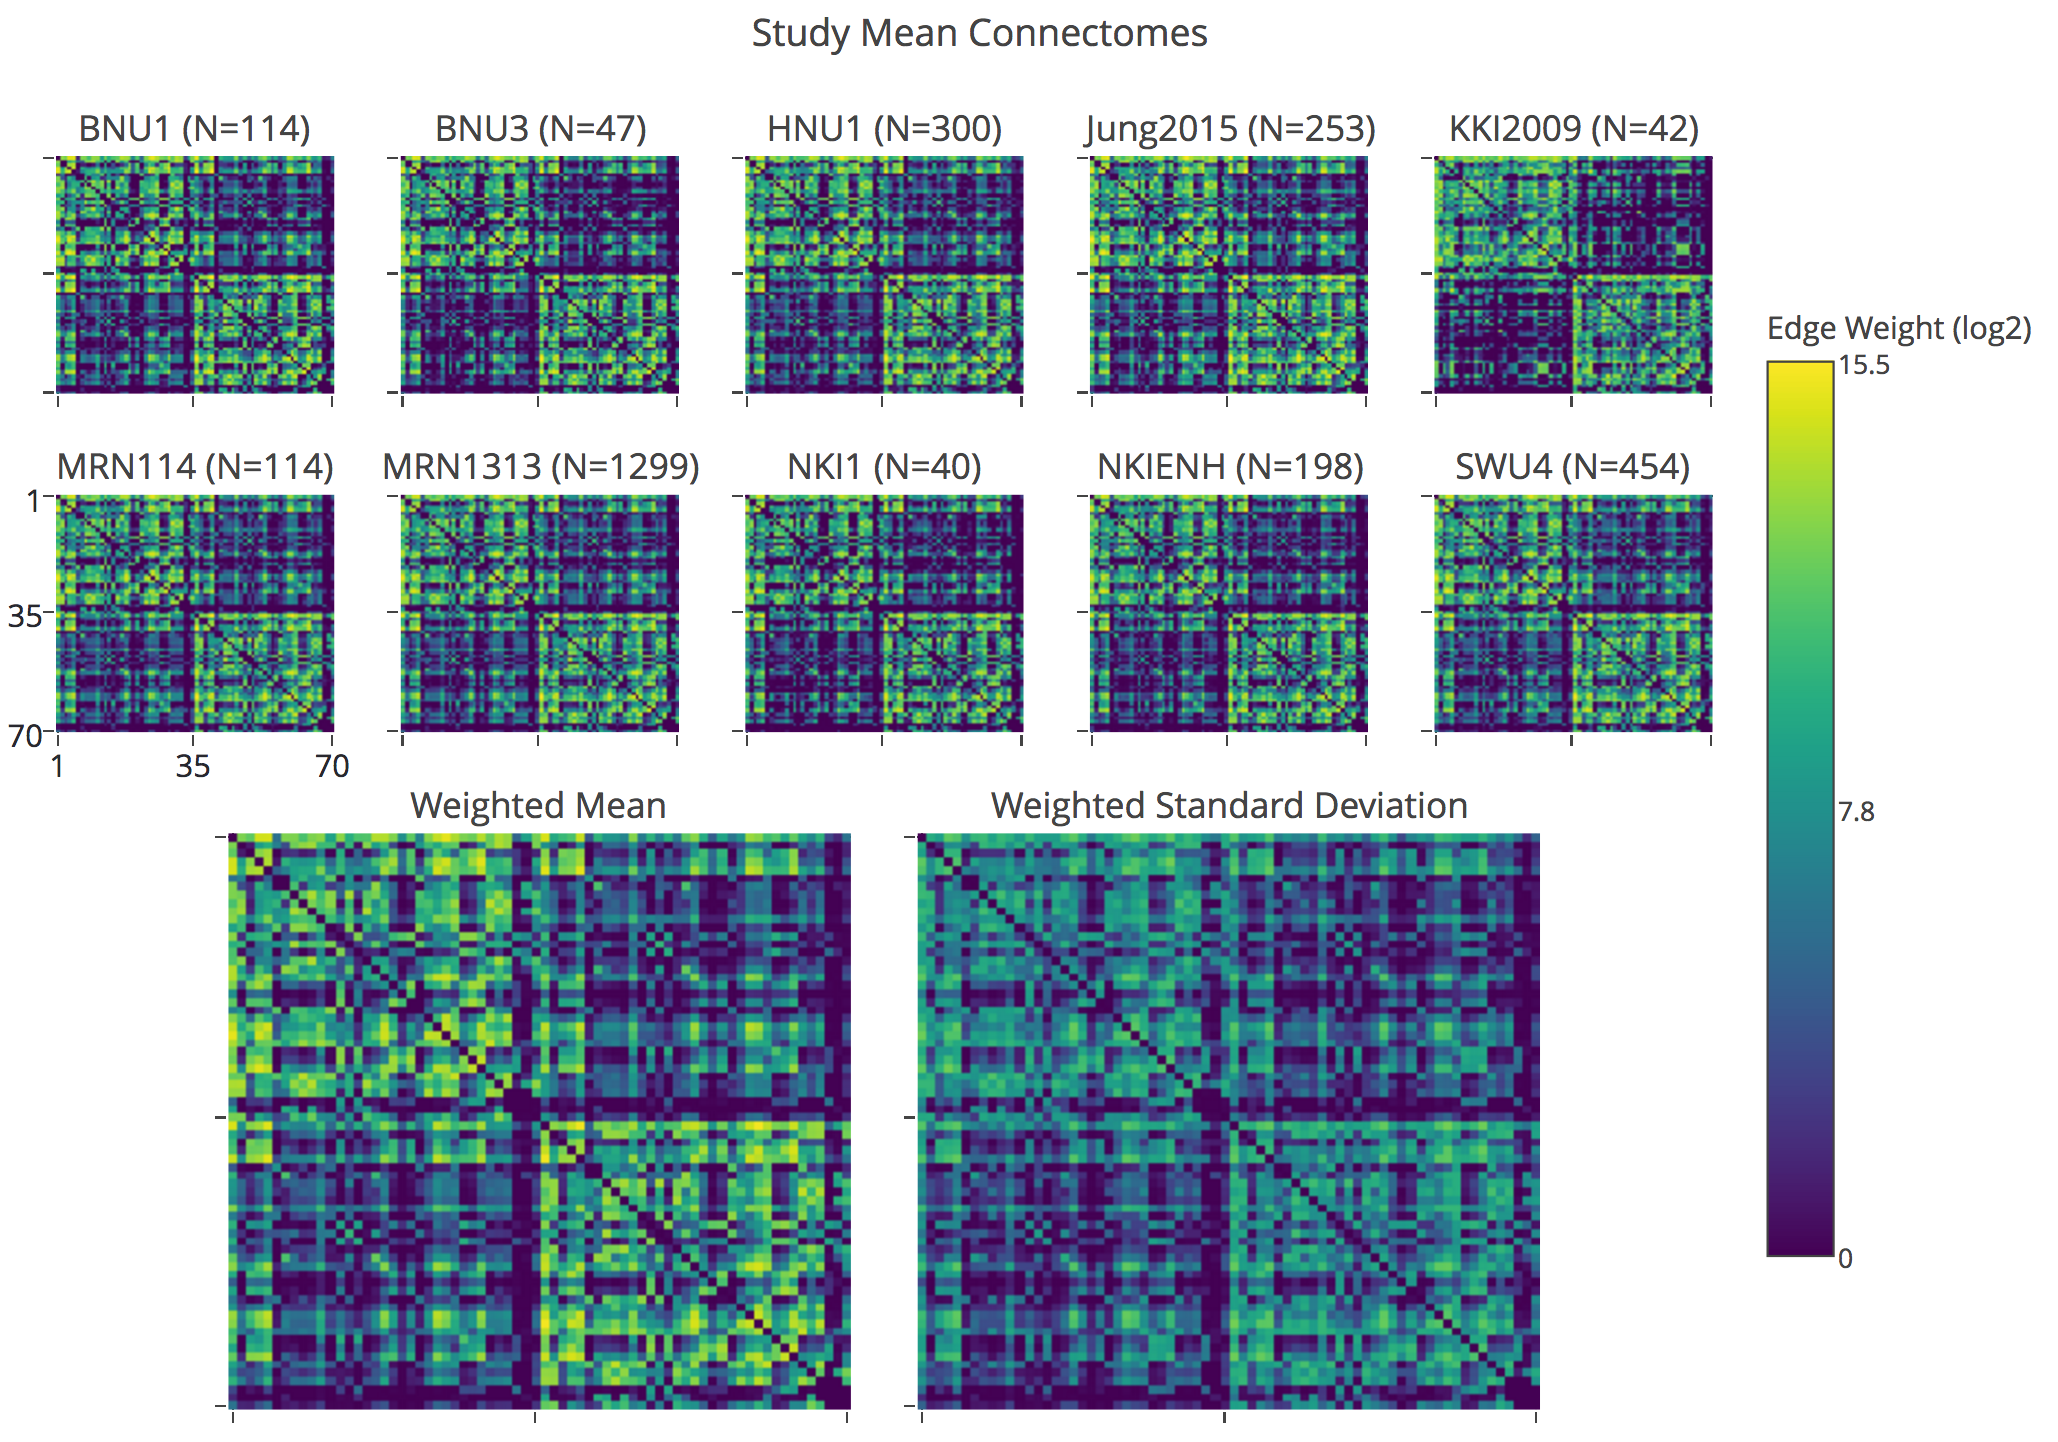
\includegraphics[width=\textwidth]{../../figs/fig_meanconnectome.png}
\end{subfigure}
\caption{\textbf{Multi-Study Mean Connectomes}. Looking at 70-nodes graphs built upon the Desikan parcellation, we have
computed the mean connectome from a variety of processed datasets. We then computed a weighted mean and standard
deviation of the mean connectomes to produce the largest known population-level connectome to-date, consisting of 2861
sessions. As expected, ipsi-lateral connectivity is consistently more dense than contra-lateral connectivity.
Similarly, the standard deviation connectome, which highlights edges that are more highly variable, shows higher
ipsi-lateral density. This suggests that not only are same-hemisphere connections more likely to occur, but they have
a higher variance than across-hemisphere connections, as well.}
\label{fig:mean}
\end{cframed}
\end{figure}

\end{document}
